\documentclass{article}

\usepackage{tikz} 
\usetikzlibrary{automata, positioning, arrows} 

\usepackage{amsthm}
\usepackage{amsfonts}
\usepackage{amsmath}
\usepackage{amssymb}
\usepackage{fullpage}
\usepackage{color}
\usepackage{parskip}
\usepackage{hyperref}
  \hypersetup{
    colorlinks = true,
    urlcolor = blue,       % color of external links using \href
    linkcolor= blue,       % color of internal links 
    citecolor= blue,       % color of links to bibliography
    filecolor= blue,        % color of file links
    }
    
\usepackage{graphicx}
\usepackage{listings}
\usepackage[utf8]{inputenc}                                                    
\usepackage[T1]{fontenc}                                                       

\definecolor{dkgreen}{rgb}{0,0.6,0}
\definecolor{gray}{rgb}{0.5,0.5,0.5}
\definecolor{mauve}{rgb}{0.58,0,0.82}

\lstset{frame=tb,
  language=haskell,
  aboveskip=3mm,
  belowskip=3mm,
  showstringspaces=false,
  columns=flexible,
  basicstyle={\small\ttfamily},
  numbers=none,
  numberstyle=\tiny\color{gray},
  keywordstyle=\color{blue},
  commentstyle=\color{dkgreen},
  stringstyle=\color{mauve},
  breaklines=true,
  breakatwhitespace=true,
  tabsize=3
}

\newtheoremstyle{theorem}
  {\topsep}   % ABOVESPACE
  {\topsep}   % BELOWSPACE
  {\itshape\/}  % BODYFONT
  {0pt}       % INDENT (empty value is the same as 0pt)
  {\bfseries} % HEADFONT
  {.}         % HEADPUNCT
  {5pt plus 1pt minus 1pt} % HEADSPACE
  {}          % CUSTOM-HEAD-SPEC
\theoremstyle{theorem} 
   \newtheorem{theorem}{Theorem}[section]
   \newtheorem{corollary}[theorem]{Corollary}
   \newtheorem{lemma}[theorem]{Lemma}
   \newtheorem{proposition}[theorem]{Proposition}
\theoremstyle{definition}
   \newtheorem{definition}[theorem]{Definition}
   \newtheorem{example}[theorem]{Example}
\theoremstyle{remark}    
  \newtheorem{remark}[theorem]{Remark}

\title{CPSC-406 Report}
\author{Sami Hammoud  \\ Chapman University}

\date{\today} 

\begin{document}

\maketitle

\begin{abstract}
\end{abstract}

\setcounter{tocdepth}{3}
\tableofcontents

\section{Introduction}\label{intro}

\section{Week by Week}\label{homework}

\subsection{Week 1}

\subsubsection*{Exercise 1}
Consider the following DFAs $\mathcal{A}_1$ and $\mathcal{A}_2$.

\begin{figure}[ht]
  \centering
  % DFA A1: 4 states, state 3 accept, state 4 trap
  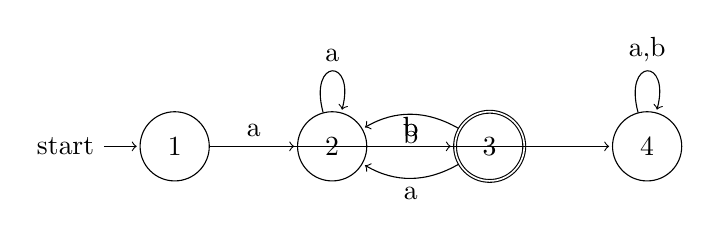
\begin{tikzpicture}[shorten >=1pt, node distance=2cm, auto]
    \node[state, initial] (1) {1};
    \node[state, right of=1] (2) {2};
    \node[state, accepting, right of=2] (3) {3};
    \node[state, right of=3] (4) {4};
    \path[->] (1) edge node {a} (2) (1) edge node {b} (4)
              (2) edge[loop above] node {a} (2) (2) edge node {b} (3)
              (3) edge[bend left] node {a} (2) (3) edge[bend right] node {b} (2)
              (4) edge[loop above] node {a,b} (4);
  \end{tikzpicture}
  \hspace{2cm}
  % DFA A2: 3 states, state 3 accept
  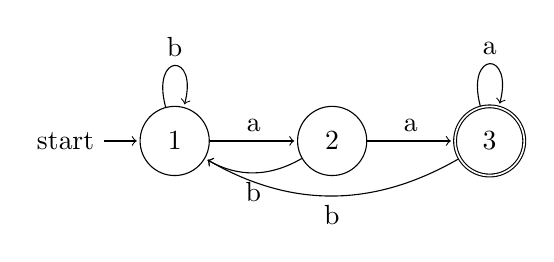
\begin{tikzpicture}[shorten >=1pt, node distance=2cm, auto]
    \node[state, initial] (1) {1};
    \node[state, right of=1] (2) {2};
    \node[state, accepting, right of=2] (3) {3};
    \path[->] (1) edge node {a} (2) (1) edge[loop above] node {b} (1)
              (2) edge node {a} (3) (2) edge[bend left] node {b} (1)
              (3) edge[loop above] node {a} (3) (3) edge[bend left] node {b} (1);
  \end{tikzpicture}
  \caption{DFAs $\mathcal{A}_1$ (left) and $\mathcal{A}_2$ (right).}
  \label{fig:dfas}
\end{figure}

Complete the following table with all 8 possible strings of length 3 over $\{a,b\}$:

\begin{center}
\begin{tabular}{|c|c|c|}
  \hline
  \textbf{String} & \textbf{Accepted by $\mathcal{A}_1$?} & \textbf{Accepted by $\mathcal{A}_2$?} \\
  \hline
  aaa & No & Yes \\
  aab & Yes & No \\
  aba & No & No \\
  abb & No & No \\
  baa & No & Yes \\
  bab & No & No \\
  bba & No & No \\
  bbb & No & No \\
  \hline
\end{tabular}
\end{center}

\section{Synthesis}

\section{Evidence of Participation}

\section{Conclusion}\label{conclusion}

\begin{thebibliography}{99}
\bibitem[BLA]{bla} Author, \href{https://en.wikipedia.org/wiki/LaTeX}{Title}, Publisher, Year.
\end{thebibliography}

\end{document}
